\documentclass[aip,pop,amsmath,amssymb,peprint,superscriptaddress]{revtex4-1} %preprint version
\usepackage{graphicx}% Include figure files
\usepackage{dcolumn}% Align table columns on decimal point
\usepackage{bm}% bold math

    \renewcommand{\topfraction}{0.9}    % max fraction of floats at top
    \renewcommand{\bottomfraction}{0.8}    % max fraction of floats at bottom
    \setcounter{topnumber}{2}
    \setcounter{bottomnumber}{2}
    \setcounter{totalnumber}{4}     % 2 may work better
    \setcounter{dbltopnumber}{2}    % for 2-column pages
    \renewcommand{\dbltopfraction}{0.9}    % fit big float above 2-col. text
    \renewcommand{\textfraction}{0.07}    % allow minimal text w. figs
    \renewcommand{\floatpagefraction}{0.7}    % require fuller float pages
    \renewcommand{\dblfloatpagefraction}{0.7}    % require fuller float pages
    \setlength{\abovecaptionskip}{5pt}
    \setlength{\belowcaptionskip}{5pt}
    \setlength{\parskip}{0pt}
    \setlength{\textfloatsep}{5pt} 

\begin{document}
\title{Turbulence and transport suppression scaling with flow shear on the Large Plasma Device}
\author{D.A. Schaffner}
\author{T.A Carter}
\author{G.D. Rossi}
\author{D.S. Guice}
\author{J.E. Maggs}
\author{S. Vincena}
\author{B. Friedman}
\affiliation{Department of Physics and Astronomy, University of California, Los Angeles}
\date{\today}
\begin{abstract}
Continuous control over azimuthal flow and shear in the edge of the
Large Plasma Device (LAPD) [W. Gekelman, \textit{et. al},
  Rev. Sci. Instr. \textbf{62}, 2875 (1991)] has been achieved using a
biasable limiter.  This flow control has allowed a careful study of
the effect of flow shear on pressure-gradient-driven turbulence and
particle transport in LAPD. The combination of externally-controllable
shear in a turbulent plasma along with the detailed spatial diagnostic
capabilities on LAPD makes the experiment a useful testbed for
validation of shear suppression models. Motivated by these models,
power-law fits are made to the density and radial velocity fluctuation
amplitudes, particle flux, density-potential crossphase and radial
correlation length.  The data show a break in the trend of these
quantities  when the shearing rate ($\gamma_s = \partial
V_\theta/\partial r$) is comparable to the turbulent decorrelation
rate ($1/\tau_{\rm ac}$).  No one model captures the trends in the
all turbulent quantities for all values of  the shearing rate, but
some models successfully match the trend in either the weak
($\gamma_s \tau_{\rm ac} < 1$) or strong ($\gamma_s \tau_{\rm ac} >
1$) shear limits. 
\end{abstract}
\maketitle

\section{Introduction}

Suppression of turbulence and turbulent transport by flow shear has
been observed on a multitude of different magnetized plasma
experiments~\cite{burrell97,burrell99,terry00,oost03,sakai93,maggs07,carter09,schaffner12}. While
the importance of cross-field flow shear for the successful high
confinement operation of fusion devices is well
recognized~\cite{burrell92,wagner07}, we still lack a fully first-principles
understanding of how sheared flow regulates turbulence and transport.
This understanding is essential in the development
of a predictive capability for transport for current and future
devices such as ITER. Experimental validation of shear suppression
models is a critical part of this development process, providing
motivation for experiments in which the response of turbulence to
shear flow is carefully documented.  External control of flow shear in
a magnetized plasma has been previously achieved in a number of
torodial devices using biased electrodes to drive cross-field currents
and provide torque to drive plasma
rotation~\cite{taylor89,weynants92}.   Transport reduction and
confinement transitions have been observed in response to biasing and
this response has been compared to models for shear suppression, in
particular in work performed by the TEXTOR group~\cite{weynants98,boedo00,boedo02}.

Biasing has been used to induce rotation and cause transitions in particle
confinement in the Large Plasma Device
(LAPD)~\cite{maggs07,carter09}. Recently, a new data set has been
gathered on LAPD in which the flow shear was continuously varied using
a biasable limiter~\cite{schaffner12}. These experiments demonstrated
shear suppression of turbulent transport and provided measurements of a number of turbulent quantities including cross-field particle flux, density and radial $E\times B$ velocity fluctuations, density-velocity crossphase, and radial correlation length. Moreover, the scan included data points in both the weak and strong shear regime, as defined by the ratio of shearing rate to inverse autocorrelation time.  This provides the ability for comparison to models which make separate predictions for each regime.

Models based on radial decorrelation of turbulent structures by
sheared flow are prevalent in the theoretical literature~\cite{biglari90,shaing90,zhang92,zhang93,ware96,ware98,terry01,kim03,kim04,newton11} and provide a
number of predictions concerning the quantitative scaling of turbulent
quantities with shear. The basic premise underlying these models is the competition between linear or nonlinear turbulence
dynamics and the tendency of sheared flows to ``rip apart'' or
decorrelate turbulent structures; this leads to reduced
fluctuation amplitude and decreased radial transport step-size. A
large number of theoretical models have been developed which use this
underlying principle. Variation in the predictions of these models
arise from assumptions: strength of flow shear compared to turbulence
timescales (strong vs weak), the underlying instability driving the
turbulence (i.e. Ion Temperature Gradient (ITG) or Resistive Pressure
Gradient Driven Turbulence (RPGDT)), as well as consideration of passive versus dynamic scalars. 

This paper presents experimental fits of density fluctuation
amplitude, radial velocity fluctuation amplitude, particle flux,
crossphase, diffusivity and radial correlation length as functions of
flow shear and compares them to a number of model predictions. No one
model predicts how all the quantities scale with shearing rate though
some models do make favorable comparisons for some quantities.  The
data generally show a stronger decrease in turbulent fluctuations than
crossphase as a contributer to reduction of particle flux.  Fits to
the variation of the experimentally computed diffusion coefficient
with shear compare well to numerical simulation predictions. 

This paper is organized as follows.  A brief review of shear decorrelation models is provided in Section II, followed by a discussion of the LAPD experiments in Section III. In Section IV, the approach for model fitting of the experimental data is discussed and the results of these fits are presented in Section V. Finally a discussion of how these fits compare to analytic and simulation model predictions is given in Section VI.

\section{Models of Shear Suppression}

The models presented here predict the suppression of various quantities as functions of shearing rate, $\gamma_{s} = d/dr(V_{\theta})$, normalized to the autocorrelation time, or decorrelation time, $\tau_{ac}$.

Two of the earliest models of shear suppression were decorrelation models developed by Biglari, Diamond, Terry~\cite{biglari90} (hereafter BDT) and Shaing~\cite{shaing90}. The BDT theory presents a generalized analysis of the transport of a passive scalar in a mean sheared flow in the strong-shear regime with constant turbulent drive (pressure gradient). The BDT model predicts that normalized fluctuation amplitude scales directly with shear to the -2/3 power:
%
\begin{equation}
\frac{\langle |\tilde{\xi}|^{2} \rangle}{\langle |\tilde{\xi}|^{2} \rangle}_{\gamma_{s}=0} \sim (\gamma_{s}\tau_{ac})^{-2/3}
\label{eq:BDT_theory}
\end{equation}
%
where $\xi$ can be any quantity such as density or temperature. Conversely, the Shaing model focuses on the weak shear limit and predicts a scaling of the form:
%
\begin{equation}
\frac{\langle |\tilde{\xi}|^{2} \rangle}{\langle |\tilde{\xi}|^{2} \rangle}_{\gamma_{s}=0} \sim 1- \alpha(\gamma_{s}\tau_{ac})^2
\label{eq:shaing_theory}
\end{equation}
%
where $\alpha$ is a constant containing mode number information. 

Zhang and Mahajan~\cite{zhang92,zhang93} developed a model which
included the self-consistent modification of the fluctuation spectrum
and the diffusion coefficient by flow shear.  This allowed the
development of a model for shear suppression of turbulent amplitude which could span both the weak and strong shear regimes:
%
\begin{equation}
\left(\frac{\langle |\tilde{\xi}|^{2} \rangle}{\langle |\tilde{\xi}|^{2} \rangle}_{\gamma_{s}=0}\right)^{-1} \sim 1+\alpha(\gamma_{s}\tau_{ac})^2
\label{eq:zm_theory}
\end{equation}
%
The resulting model shows correspondence to the Shaing model in the weak shear regime while the BDT model can be recovered in the strong shear regime but only for the case where the diffusion coefficient is constant (independent of fluctuation amplitude).

Work by Ware and Terry~\cite{ware96,ware98} made predictions for the
effect of shear on particle transport specifically in resistive
pressure-gradient driven turbulence (RGPDT). Their work predicted a decrease in flux as $\Gamma_{p} \sim 1-\gamma_{s}^2$ in the weak shear limit.  Additionally,  the model predicted a decrease in the cosine of the crossphase between density and radial velocity fluctuations of the form $1-\gamma_{s}^2$. They too incorporated the modification of the pressure gradient, formulating an expression for shear suppression of radial particle diffusivity of the form:
%
\begin{equation}
\frac{D}{D_{\gamma_{s}=0}} \sim 1-\beta(\gamma_{s})^2
\label{eq:ware_diff_theory}
\end{equation}
%
where $\beta$ is a constant which depends on the linear growth rate and radial mode width.

Further work by Terry, Newman and Ware~\cite{terry01} examined the modification of flux in the strong shear regime for a non-mode-specific turbulent system, predicting a direct scaling of $\Gamma_{p} \sim \gamma_{s}^{-4}$ overall.  Here fluctuation amplitude reduction contributed one power while crossphase reduction contributed three powers of $\gamma_s$, indicating that, in the strong shear limit, crossphase modification is the dominant flux suppression mechanism rather than reduction of the fluctuation amplitude. 

Kim and Diamond~\cite{kim03} recast the decorrelation model to include resonance absorption between the shear flow and fluctuations leading to a much weaker dependence of particle flux on shear, $\Gamma_{p} \sim \gamma_{s}^{-1}$, and even weaker dependence of the crossphase on shear: $\cos(\theta_{nv_{r}}) \sim \gamma_{s}^{-1/6}$.  In this model, fluctuations decreased as $|\tilde{n}|^{2} \sim \gamma_{s}^{-5/3}$. Additional work along these lines~\cite{kim04} considered a more self-consistent model for the turbulence, treating the fluctuating flows dynamically using interchange drive.  This model predicted a decrease in fluctuating radial velocity amplitude as a function of shear which scales as $|\tilde{v_{r}}|^{2} \sim \gamma_{s}^{-3}$ in the weak shear limit, and as $|\tilde{v_{r}}|^{2} \sim \gamma_{s}^{-4}$ in the strong-shear limit.

Finally, work by Newton and Kim has utilized numerical simulations
using a generic turbulence model~\cite{newton11} with a finite
correlation time, $\tau_{ac} \geq \gamma_{s}^{-1}$. Their work produced scalings of $D \sim \gamma_{s}^{-1.75}$, $|\tilde{n}|^{2} \sim \gamma_{s}^{-2.41}$, and $\cos(\theta_{nv_{r}}) \sim \gamma_{s}^{-0.22}$ which correspond to the strong shear regime for this dataset.

\section{Shear Suppression Experiments}

The Large Plasma Device (LAPD) is a 17m long, $\sim$60cm diameter cylindrical plasma produced by a barium-oxide coated nickel cathode~\cite{gek91}. In the experiments reported here, a plasma of density $\sim$$2 \times 10^{12}$ cm$^{-3}$ and peak temperature of ~8eV is produced in a uniform solenoidal magnetic field of 1000G. All measurements reported here were collected using Langmuir probes recording floating potential, $V_{f}$, or ion saturation current, $I_{\rm sat}$. Azimuthal electric field fluctuations, $\tilde{E}_{\theta}$, are found by taking the simultaneous difference in two $V_{f}$ signals separated a small azimuthal distance apart. Turbulent particle flux $\Gamma \propto \left<\tilde{n}_e \tilde{E}_\theta\right>$ is determined through correlating density fluctuations with $\tilde{E}_{\theta}$ where it is assumed that $E_{\theta}$ produces radial $E \times B$ flow. The relative crossphase between fluctuation time-series is determined through the cross-spectrum of the quantities. That is,
%
\begin{equation}
\theta = \tan^{-1}\frac{\langle Q(f,r)\rangle_{f,r}}{\langle C(f,r)\rangle_{f,r}}
\label{eq:crossphase}
\end{equation}
%
where Q and C are the imaginary and real parts of the cross-spectrum, calculated from the product of the complex FFTs of the two time-series in question as in,
\begin{equation}
G(f,r) = \hat{x}^{\ast}(f,r)\hat{y}(f,r)
\label{eq:crossspectrum}
\end{equation}
%
The cross-spectrum is first averaged over frequencies to power-weight the crossphase signal, and then averaged radially, before the phase is determined using ~\ref{eq:crossphase}. Finally, steady-state azimuthal flow, $V_{\theta}$ is determined through the radial derivative of plasma potential profiles measured using a swept-Langmuir probe technique again assuming only $E \times B$ flow. The shearing rate is computed as $\gamma_{s} = d/dr(V_{\theta})$. The normalization, $\tau_{ac}$, is determined by finding the width of the autocorrelation function of the density time series at zero shearing rate. FFT quantities are calculated over a time range of 3.2ms. The plasma potential is determined from voltage sweeps 2.5ms long.

A large annular aluminum limiter was installed in LAPD to provide a parallel boundary condition for the edge plasma and is biased relative to the cathode of the plasma source to control plasma potential and cross-field flow.  A diagram of the limiter arrangement and biasing circuit is shown in Fig.~\ref{fig:velocity_flowshear}(a).

\begin{figure}[!htbp]
\centerline{
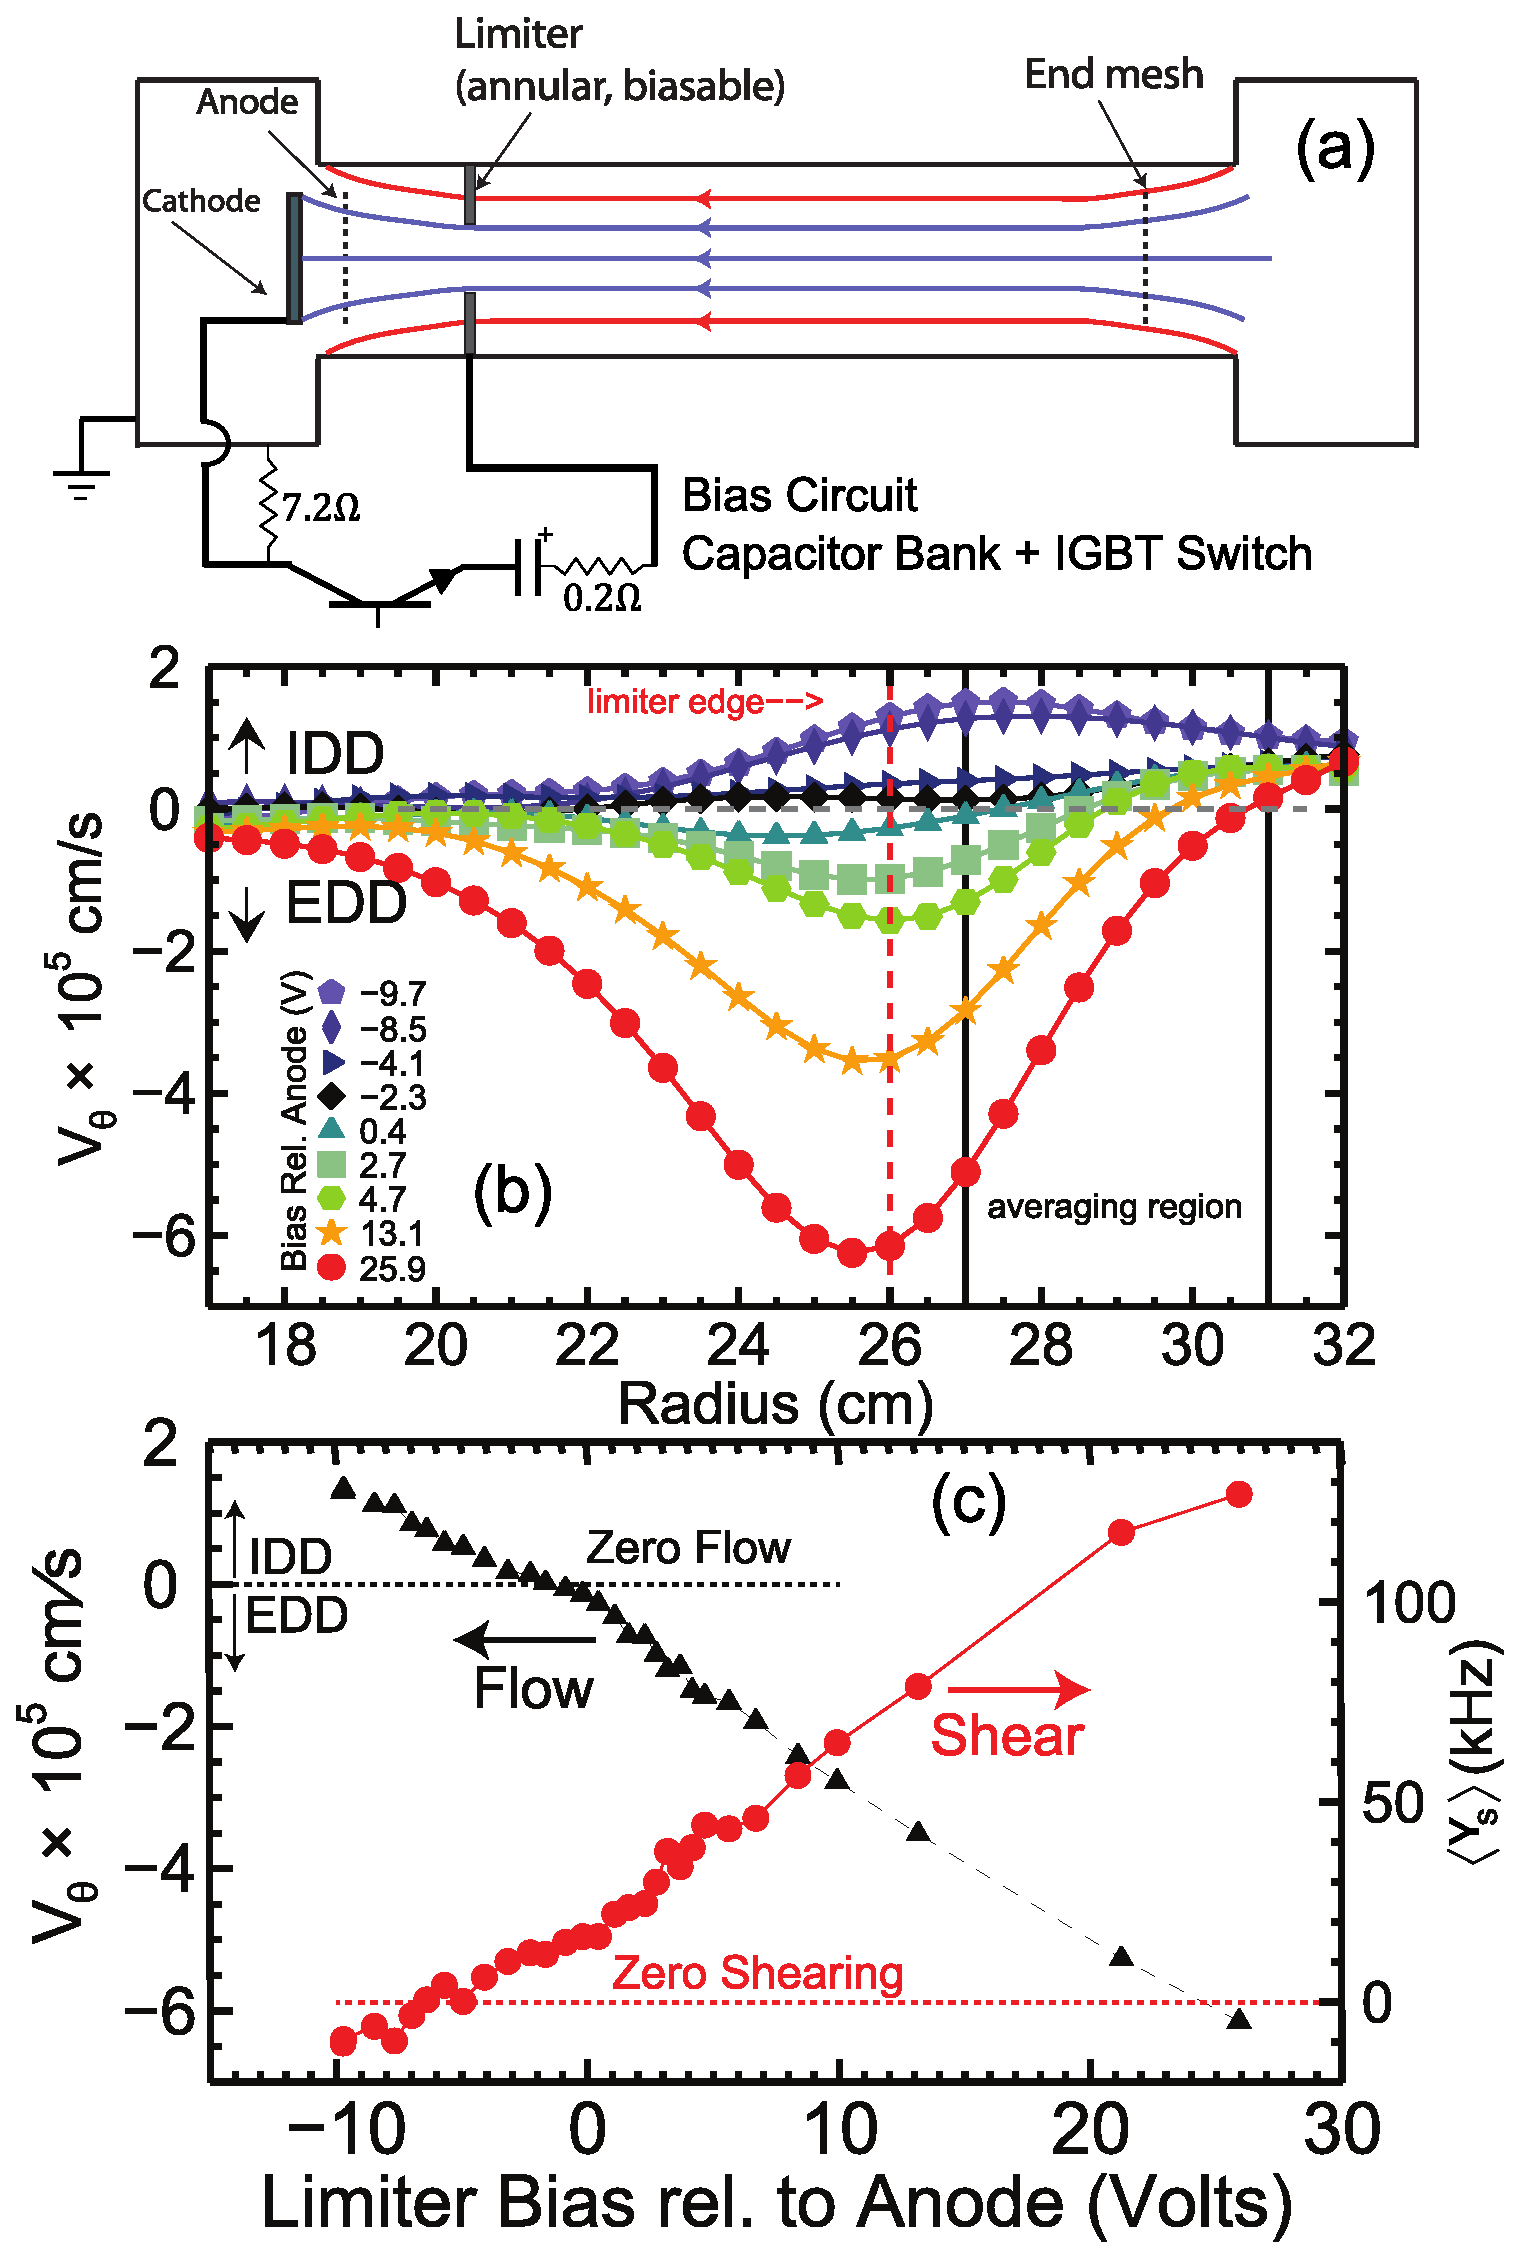
\includegraphics[width=8.5cm]{figure1.eps}}
\caption{\label{fig:velocity_flowshear} (Color online) (a) Diagram of the LAPD device showing relative location of the annular limiter and basic biasing setup.  (b) Velocity profiles using plasma potential from swept measurements. (c) Flow at the limiter edge (black, triangles) and mean shearing rate, averaged over $27 < r < 31$cm (red, circles).}
\end{figure}

A recent experiment on the LAPD demonstrated the ability to achieve
continuous control of steady-state azimuthal flow and flow shear
through the use of these biasable
limiters~\cite{schaffner12}. Spontaneous rotation is observed in LAPD
in the ion diamagnetic drift direction (IDD).  This spontaneous flow can be
reduced and reversed into the electron diamagnetic drift direction (EDD) as the
limiter bias is increased. This results in a continuous variation of
edge flow and flow shear including zero flow and flow shear
states. Shearing rates are achieved up to about five times the
turbulent inverse autocorrelation time or decorrelation time---$\tau_{ac}^{-1}$---as measured
in the state with minimum shearing rate. Radial particle flux and
fluctuation amplitude are reduced as shearing rate is increased and
the resulting transport changes cause observable steepening of the
density gradient. Figure~\ref{fig:densvrcp} shows the experimental
results for measurements of density fluctuation amplitude, radial
velocity fluctuation amplitude and density-radial velocity crossphase as functions
of normalized shearing rates. The shearing rates achieved span two
regimes: a weak-shear regime where $\gamma_{s}\tau_{ac} < 1$ and a
strong-shear regime where $\gamma_{s}\tau_{ac} > 1$. The blue solid
lines correspond to the best fits for the strong-shear cases while the
green are the best fits for the weak-shear case.  Similar plots for
particle flux and diffusivity $D = \Gamma/|\nabla n|$ are shown in
Figure~\ref{fig:fluxandD}. All data presented is averaged over the radial range $27 < r < 31$cm as indicated in Figure~\ref{fig:velocity_flowshear}. Error bars of +/-20\% for each quanitity are
shown on the plots and used in the fits, reflecting a statistical
error from the number of shots used to average the quantity ($\sigma
\sim 1/\sqrt{\rm N_{shots}}$). 

Measurements of the radial correlation length were recorded as a function of shearing rate (applied bias) using a two-probe correlation technique. A reference probe collecting $I_{\rm sat}$ is kept stationary at a particular axial and radial location within LAPD. A second Langmuir probe situated at an axial point closer to the cathode is moved shot-to-shot in a rectangular grid around the radial location of the reference probe.  The cross-field cross-correlation function of these two measurements is computed shot-to-shot for a delay time $\tau$ as $C(x,y,\tau) = \langle I_{\rm ref}(x,y,t)I_{\rm mot}(x,y,t+\tau)\rangle$.

Figure~\ref{fig:radcorr}(a) shows the normalized correlation function $C(x,y)/C_{\rm max}$ for the unbiased state (flow in the IDD), a minimum shear state, and a high bias state (large EDD flow) with a reference probe located at $x=29.5$cm, $y=0$cm (right in the middle of the shear layer). The black curve represents the contour line where $C(x,y)/C_{\rm max} = 0.5$. The radial correlation length $\Delta r_{c}$ is defined here as the radial width of this black curve through the reference probe location.   The variation of the correlation length versus shearing rate is shown in Figure~\ref{fig:radcorr} (normalized to the maximum radial correlation length calculated for all biases, $r_max = 5.5$cm).
The correlation length is found to decrease substantially with shear.  A break in the trend of decreasing correlation length is observed for larger shearing rates where the correlation function appears to be dominated by a coherent mode (which also appears in the temporal power spectrum).

Some achieved parameter regimes for the shearing rate and density
gradient length scales are presented in Figure~\ref{fig:LgammaLn}. The
azimuthal velocity scale length is calculated as $L_{v} = |\nabla
\ln(v_{E\times B})|^{-1}$. This value is compared to the density
gradient scale length, $L_{n} = |\nabla \ln{n}|^{-1}$ as a function of
normalized shearing rate. This plot shows that for the all of the
strong shear regime, and nearly half of the weak shearing regime,
$L_{n} > L_{v}$. The reverse is true only for the weakest shear. In
general, the velocity gradient scale length decreases much faster than the density gradient scale length with increased shearing rate magnitude and is smaller than the density gradient scale length for most of the dataset.

\section{Experimental Shear Suppression Scaling}

\begin{figure}[!htbp]
\centerline{
\includegraphics[width=8.5cm]{figure2.eps}}
\caption{\label{fig:densvrcp} (Color online) Scaling of (a)density fluctuation amplitude, (b)radial velocity fluctuation amplitude, and (c)density-radial velocity crossphase. Density and velocity fluctuations are each normalized to the value measured at minimum shear. The green curves correspond to $1-\gamma_{s}^{\nu}$ fits of the weak shear regime. The blue curves correspond to $\gamma_{s}^{\nu}$ fits. The last three points in each plot are not included in the fits do to potential influence of the coherent mode at high shearing rate.}
\end{figure}

\begin{figure}[!htbp]
\centerline{
\includegraphics[width=8.5cm]{figure3.eps}}
\caption{\label{fig:fluxandD} (Color online) Scaling of (a)radial particle flux and (b)diffusion coefficient each normalized to the value at minimum shear, $\Gamma_{p}^{0} = 1.7\times10^{16} cm^{-2}$ and $D_{0} = 36.7 m^{2}/s$. The green curves correspond to $1-\gamma_{s}^{\nu}$ fits of the weak shear regime with $\nu = 0.501$ for flux and $\nu = 0.418$ for D. The blue curves correspond to $\gamma_{s}^{\nu}$ fits with $\nu = -1.719$ for flux and $\nu = -1.646$ for D. The last three points in each plot are not included in the fits do to potential influence of the coherent mode at high shearing rate.}
\end{figure}

\begin{figure}[!htbp]
\centerline{
\includegraphics[width=8.5cm]{figure4.eps}}
\caption{\label{fig:radcorr} (Color online) Normalized correlation functions for (a)unbiased, IDD flow state, (b)no shear state, and (c)high bias, high EDD flow state where the black curve represents a decrease of 0.5 from peak. (Color scale indicates correlation for all three biases). (d)Radial correlation length normalized to maximum correlation length (5.5cm) versus normalized shearing rate with M2 fits for weak (green) and strong (blue) shear. (e)Ratio of radial correlation length to density gradient scale length.}
\end{figure}

\begin{figure}[!htbp]
\centerline{
\includegraphics[width=8.5cm]{figure5.eps}}
\caption{\label{fig:LgammaLn} Ratio of velocity gradient length scale
  to density gradient length scale versus normalized shearing rate in the radial region of 27 to 31cm.}
\end{figure}

\begin{figure}[!htbp]
\centerline{
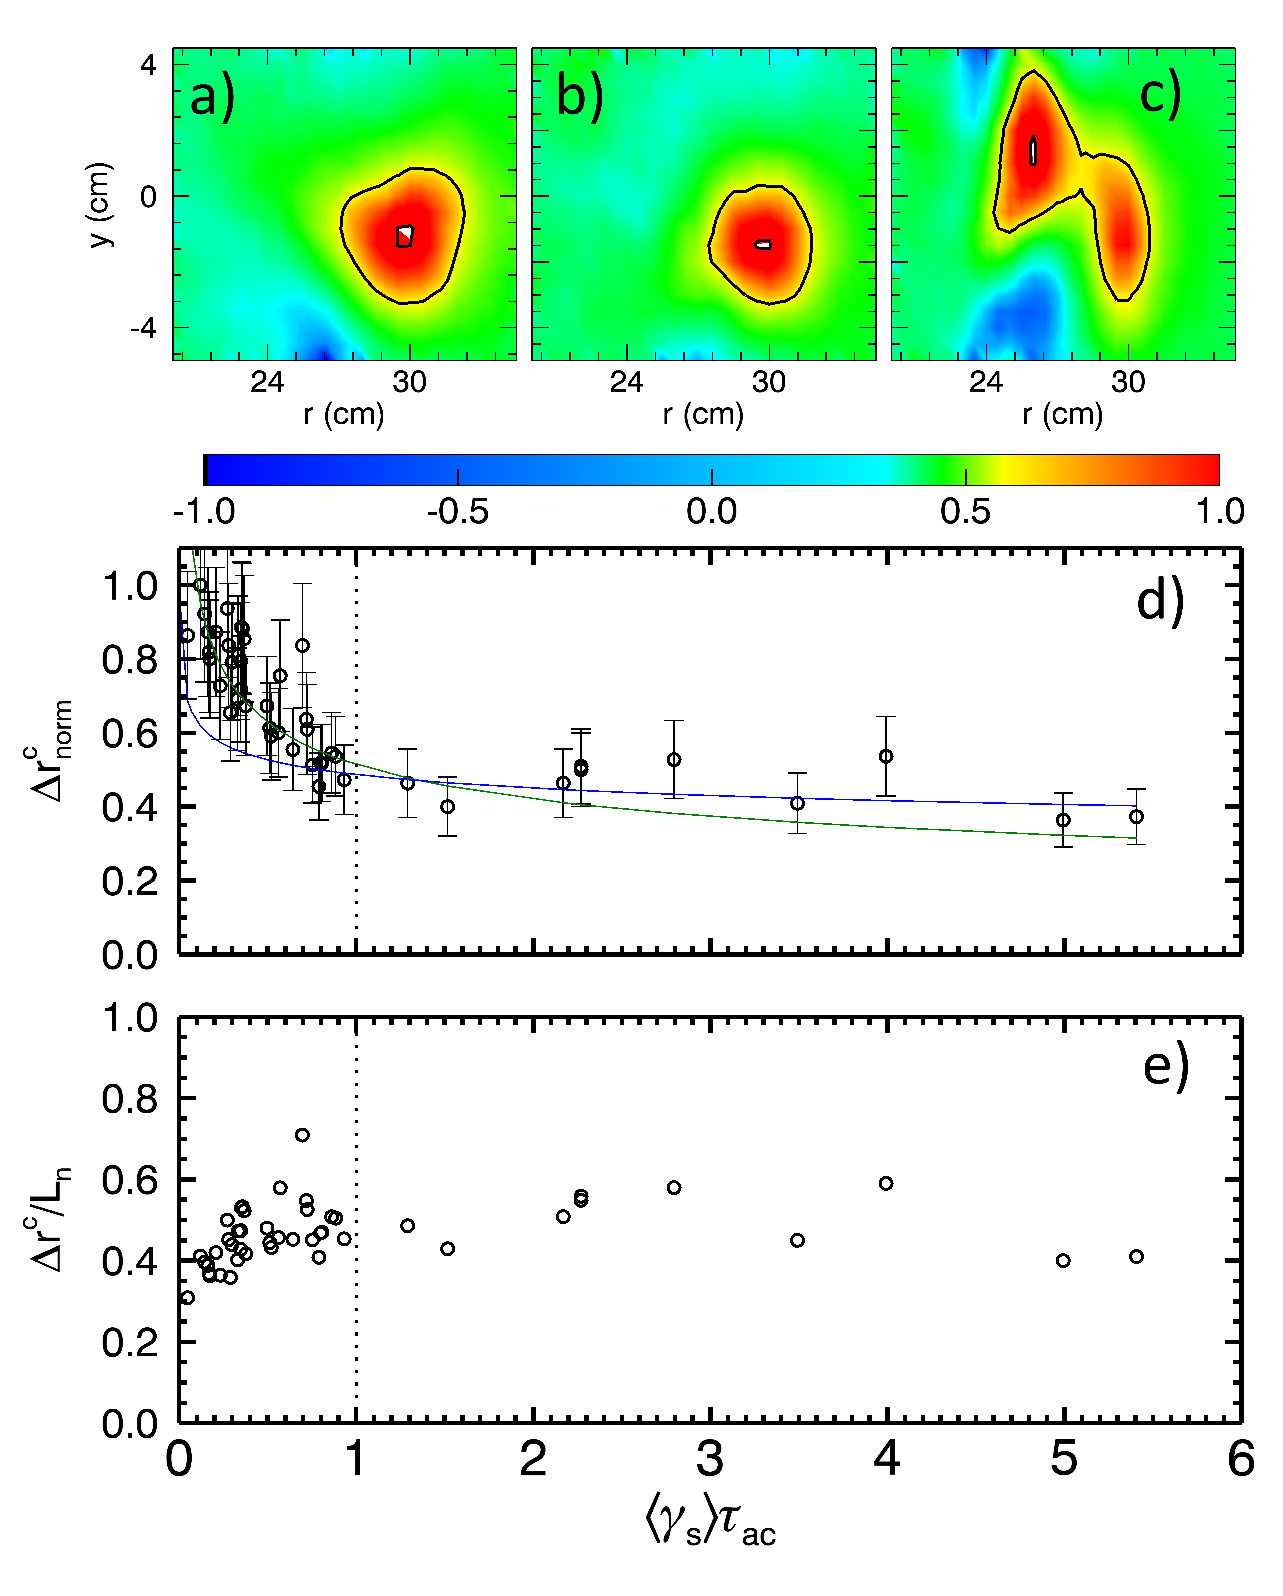
\includegraphics[width=8.5cm]{figure6.eps}}
\caption{\label{fig:densloglog_strong} (Color online) Log-Log plot of (a-b)density
  fluctuation amplitude and (c-d)particle flux versus shearing rate. Weak shear fits, (a) and (c), are shown with the solid red lines and a theoretical prediction---dashed line---of $\nu = 2$ is included for comparison of slope (line is manually offset). Strong shear fits, (b) and (d), are shown with the solid blue lines and theoretical predictions are indicated with the dashed lines. The last three points in each plot are not included in the fits do to potential influence of the coherent mode at high shearing rate}
\end{figure}

\begin{figure}[!htbp]
\centerline{
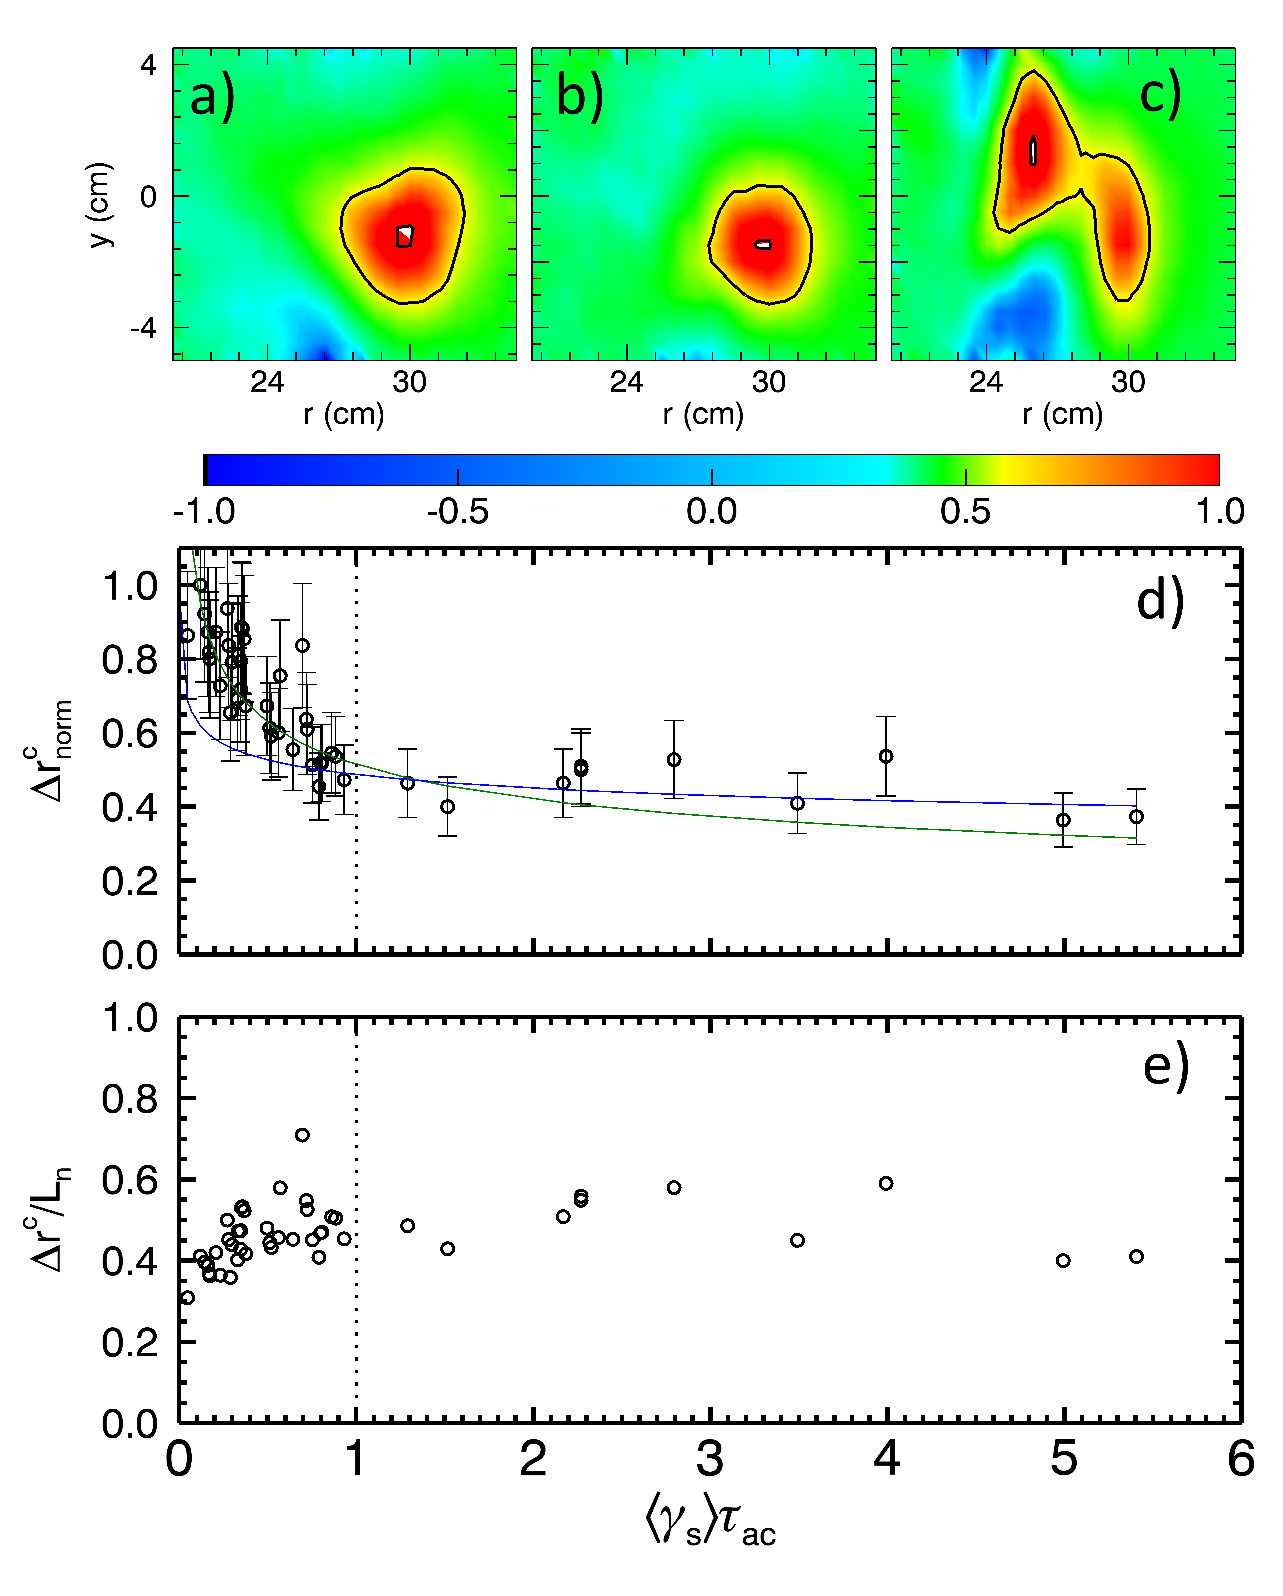
\includegraphics[width=8.5cm]{figure7.eps}}
\caption{\label{fig:fullrange_fits} (Color online) Fits over a shear range spanning both weak and strong regimes for (a) density fluctuation amplitude, (b)particle flux, (c)diffusivity, and (d)crossphase. Red lines correspond to $\sim C\gamma_{s}^{\nu}$ model while the blue curves correspond to the $\sim 1/(1+C\gamma_{s}^{\nu})$ model.}
\end{figure}

\begin{table}
\caption{\label{tab:table1}Power-law fits for $|\tilde{n}^{2}|$  with shear for frequencies in 350Hz to 100kHz. Model form is the particular model used in the fit, with C a constant and $\nu$ resulting best-fit exponent.}
\begin{ruledtabular}
\begin{tabular}{llccc}
Model form&$\gamma_{s}$ regime&$\nu$&$\chi^2$&$\chi^2/ndf$\\
\hline
$\sim 1-C\gamma_{s}^\nu$&$\gamma_{s}\tau_{ac}<1$&1.228&1.091&0.0642\\
$\sim 1-C\gamma_{s}^\nu$&$\gamma_{s}\tau_{ac}>1$&0.231&0.0332&0.0037\\
$\sim C\gamma_{s}^\nu$&$\gamma_{s}\tau_{ac}<1$&-0.116&0.1791&0.0094\\
$\sim C\gamma_{s}^\nu$&$\gamma_{s}\tau_{ac}>1$&-0.512&0.0024&0.0003\\
\end{tabular}
\end{ruledtabular}
\end{table}

\begin{table}
\caption{\label{tab:table2}Power-law fits for $|\tilde{v}_{r}^{2}|$ scaling with shear for frequencies in 350Hz to 100kHz.}
\begin{ruledtabular}
\begin{tabular}{llccc}
Model form&$\gamma_{s}$ regime&$\nu$&$\chi^2$&$\chi^2/ndf$\\
\hline
$\sim C\gamma_{s}^\nu$&$\gamma_{s}\tau_{ac}<1$&0.016&0.2121&0.0117\\
$\sim C\gamma_{s}^\nu$&$\gamma_{s}\tau_{ac}>1$&-0.866&0.0037&0.0005\\
\end{tabular}
\end{ruledtabular}
\end{table}

\begin{table}
\caption{\label{tab:table3}Power-law fits for $\Gamma_{p}$ scaling with shear for frequencies in 350Hz to 100kHz.}
\begin{ruledtabular}
\begin{tabular}{llccc}
Model form&$\gamma_{s}$ regime&$\nu$&$\chi^2$&$\chi^2/ndf$\\
\hline
$\sim 1-C\gamma_{s}^\nu$&$\gamma_{s}\tau_{ac}<1$ &0.501   &0.332    &0.0189\\
$\sim 1-C\gamma_{s}^\nu$&$\gamma_{s}\tau_{ac}>1$ &0.638   &0.923    &0.103\\
$\sim C\gamma_{s}^\nu$&$\gamma_{s}\tau_{ac}<1$   &-0.111  &0.146    &0.0077\\
$\sim C\gamma_{s}^\nu$&$\gamma_{s}\tau_{ac}>1$   &-1.719  &6.54    &0.726\\
\end{tabular}
\end{ruledtabular}
\end{table}

\begin{table}
\caption{\label{tab:table4}Power-law fits for $D = \Gamma_{p}/\nabla{n}$ scaling with shear for frequencies in 350Hz to 100kHz.}
\begin{ruledtabular}
\begin{tabular}{llccc}
Model form&$\gamma_{s}$ regime&$\nu$&$\chi^2$&$\chi^2/ndf$\\
\hline
$\sim 1-C\gamma_{s}^\nu$&$\gamma_{s}\tau_{ac}<1$ &0.418   &1.4710    &0.0817\\
$\sim 1-C\gamma_{s}^\nu$&$\gamma_{s}\tau_{ac}>1$ &0.197   &0.0016    &0.0002\\
$\sim C\gamma_{s}^\nu$&$\gamma_{s}\tau_{ac}<1$   &-0.217  &0.4200    &0.0221\\
$\sim C\gamma_{s}^\nu$&$\gamma_{s}\tau_{ac}>1$   &-1.646  &0.0187    &0.0021\\
\end{tabular}
\end{ruledtabular}
\end{table}

\begin{table}
\caption{\label{tab:table5}Power-law fits for $cos(\theta_{nv_{r}})$ scaling with shear for frequencies in 350Hz to 100kHz.}
\begin{ruledtabular}
\begin{tabular}{llccc}
Model form&$\gamma_{s}$ regime&$\nu$&$\chi^2$&$\chi^2/ndf$\\
\hline
$\sim 1-C\gamma_{s}^\nu$&$\gamma_{s}\tau_{ac}<1$ &0.226   &6.1140    &0.3320\\
$\sim C\gamma_{s}^\nu$&$\gamma_{s}\tau_{ac}<1$   &-0.020  &0.0369    &0.0019\\
$\sim C\gamma_{s}^\nu$&$\gamma_{s}\tau_{ac}>1$   &-0.365  &0.0023    &0.0003\\
\end{tabular}
\end{ruledtabular}
\end{table}

The variation of the experimentally measured quantities with normalized shearing rate was fit to functions motivated by models discussed above: functions of the form $1-\gamma_{s}^{\nu}$ (hereafter M1) and of $\gamma_{s}^{\nu}$ (hereafter M2). For M1, the measured quantity, $y$, was normalized to the value at zero shear, then transformed as $-(1-y)$. Then, taking the logarithm of both sides, a linear fit was made for points in the weak shear and in the strong shear separately. The resulting slope of the fit is taken as the power $\nu$. For M2, no transformation of the quantity $y$ is made before taking the logarithm and fitting. For a complete comparison to the wide range of model predictions made, fits were made for density fluctuation amplitude, radial particle flux, density-radial velocity fluctuation crossphase, radial velocity (ExB) fluctuation amplitude, radial correlation length, and experimentally determined diffusivity ($\Gamma/|\nabla n|$). The best fits are summarized in Table~\ref{tab:table1}-~\ref{tab:table6} for each model type and for both weak and strong shear. The $\chi^{2}$ and $\chi^{2}/$ndf (where ndf is the number of degrees of freedom) is also indicated in the tables.  For weak shear fits, all points less than the weak shear cutoff $\gamma_{s}\tau_{ac}<1$ are used in the fit. For strong shear, all but the last three points are used. The last points appear to be strongly influenced by the presence of a coherent mode that develops in the highest shear and flow cases and is thought to be a break from the scaling observed in the strong shear regime. For quantities determined by averaging over frequency (e.g. density and velocity fluctuation amplitudes, flux and diffusivity) the frequency band used was 350Hz to 100kHz.

The log-log plots highlight the break in the trend between the weak and
strong shear regimes. It should be noted that in addition to turbulent
quantities showing a different trend with shear below and above a
normalized shearing rate of unity, at the same time, the density
gradient scale length also shows a marked change in
behavior~\cite{schaffner12}.  The gradient scale length decreases
rapidly (increasing pressure-gradient drive) in the weak shear
regime followed by saturation in the strong shear regime (constant
turbulent drive with increased shear). Therefore care has to be taken in interpreting the change in the trends plotted above: it could be occurring due to a change in the shear regime but also could be due to the change in trend for the turbulence drive.

Lastly, fits were made a range of shearing rate that spanned
portions of both the weak and strong shear regimes; specifically, a
range that included all but the lowest two shearing rate values and
the three highest shearing rate values (again, dropping the last three to avoid any influence of the coherent mode). The models used are M2 and a third model based on the Zhang and Mahajan interpolated from Eqn.(~\ref{eq:zm_theory}) which was designed to describe both weak and shear scaling (hereafter M3). Fits and $\chi^{2}$ values are displayed for density fluctuation amplitude, particle flux, diffusivity, and crossphase in Table~\ref{tab:table7} and are shown plotted against the data in Figure~\ref{fig:fullrange_fits}.

\begin{table}
\caption{\label{tab:table6}Power-law fits for $\Delta r_{c}$ scaling with shear for frequencies in 350Hz to 100kHz.}
\begin{ruledtabular}
\begin{tabular}{llccc}
Model form&$\gamma_{s}$ regime&$\nu$&$\chi^2$&$\chi^2/ndf$\\
\hline
$\sim C\gamma_{s}^\nu$&$\gamma_{s}\tau_{ac}<1$ &-0.290 &5.8730 &0.1630\\
$\sim C\gamma_{s}^\nu$&$\gamma_{s}\tau_{ac}>1$ &-0.113 &3.7040 &0.3370\\
\end{tabular}
\end{ruledtabular}
\end{table}

\begin{table}
\caption{\label{tab:table7}Power law fits for all quantities over a
  range that spans both weak and strong shear. The smallest two
  shearing rate values are excluded to improve the fitting routine and
  the three highest shearing rate values are excluded to avoid effects of the coherent mode.}
\begin{ruledtabular}
\begin{tabular}{clccc}
Parameter&Model form&$\nu$&$\chi^2$&$\chi^2/ndf$\\
\hline
$\langle |\tilde{n}^{2}|\rangle$     & $\sim 1/(1+C\gamma_{s}^\nu$) &1.339   &0.9435    &0.0393\\
$\langle |\tilde{n}^{2}|\rangle$     & $\sim C\gamma_{s}^\nu$ &-0.527   &0.1280    &0.0053\\
$\langle \Gamma_{p}\rangle$          & $\sim 1/(1+C\gamma_{s}^\nu$) &1.199   &0.7899    &0.0329\\
$\langle \Gamma_{p}\rangle$          & $\sim C\gamma_{s}^\nu$ &-0.557   &0.2691    &0.0112\\
$\langle D\rangle$                   & $\sim 1/(1+C\gamma_{s}^\nu$) &1.387   &0.7375    &0.0307\\
$\langle D\rangle$                   & $\sim C\gamma_{s}^\nu$ &-0.938   &0.3490    &0.0145\\
$cos(\theta_{nv_{r}})$               & $\sim 1/(1+C\gamma_{s}^\nu$) &1.043   &3.8300    &0.1596\\
$cos(\theta_{nv_{r}})$               & $\sim C\gamma_{s}^\nu$ &-0.102   &0.0340    &0.0014\\

\end{tabular}
\end{ruledtabular}
\end{table}

\section{Results}

\subsection{Density and Velocity Fluctuations}

The best fits for scaling of density fluctuation amplitude are shown in Table~\ref{tab:table1}. For the weak shear regime, the $\chi^{2}$ values suggest M2 to be a slightly better fit to the data than M1. Though M1 is not used for prediction of strong shear scaling in the literature, a fit was made to it here for completeness; still, as with the weak shear regime, values of $\chi^{2}$ show M2 to be a better model for the strong shear regime as well.

The $\nu = -0.512$ fit for M2 in the strong shear limit is reasonably close to the BDT prediction of $-(2/3)$. However, it should be reiterated that BDT assumes a fixed turbulence drive and that in this dataset, the gradient scale length decreases substantially as shear is increased, resulting in an increase in turbulent drive.  This actually implies a stronger than BDT scaling of fluctuation amplitude suppression overall. The fit scaling is much smaller than that predicted by Kim/Diamond ($\nu = -5/3$) and Newton/Kim ($\nu = -2.41$). For M2 weak shear, the experimental fit of $\nu = -0.116$ also suggests weaker scaling than the prediction by Kim/Diamond of $-(2/3)$.

A prediction for the scaling of radial velocity fluctuation amplitude is only made by Kim and Diamond~\cite{kim04} in the dynamically evolved case. Fits, listed in Table~\ref{tab:table2}, suggest a much weaker scaling than predicted for both weak and strong shear. The weak shear fit actually shows a slight increase in fluctuation amplitude rather than a $\nu = -3$ scaling while in the strong shear regime a fit of $\nu = -0.866 << -4$ is found.

From fits over the full range of shearing rates, shown in Table~\ref{tab:table7}, M2 appears to be a slightly better model than M3. The M2 fit, $\nu = -0.527$, is similar to the strong shear only fit, but clearly has a worse $\chi^{2}$ value.

\subsection{Flux and Diffusivity}

Particle flux and diffusivity fits and $\chi^{2}$ results are shown in Table~\ref{tab:table3} and ~\ref{tab:table4} respectively. Like density fluctuations, M2 seems to be slightly better than M1 for fitting data in the weak shear limit based on $\chi^{2}$ values.  However, for strong shear, the M1 model actually has a much lower $\chi^{2}$ the M2 model, though M1 is not derived in the strong shear limit in the literature. Despite the higher $\chi^{2}$, the fit of $\nu = -1.719$ falls in between the extremes of predictions of $\nu = -1$ and $\nu = -4$. The weak shear fit of $\nu = -0.111$ falls far short of the Kim/Diamond M2 prediction of $\nu = -1$. In addition to being the less well-fitted model, the predicted exponent for M1 in the weak shear limit is also far less than the Terry and Ware value of $\nu = 2$.

Diffusivity, like flux, has lower $\chi^{2}$ values for M2 with weak shear and for M1 with strong shear. The only predictions for $D$ come from Terry and Ware with a functional form like M1 and a numerical simulation result from Newton and Kim~\cite{newton11} for evolved turbulence with a finite correlation time. The experimental fit of $\nu = 0.418$ again falls short of the Terry/Ware predicted $\nu = 2$, though the M2 fit in the strong shear limit with $\nu = -1.646$ is fairly close to the Newton/Kim predicted value of $\nu = -1.75$.

The full range results for flux and diffusivity again suggest a better fit for M2 over M3 and an even better fit for M2 than in the strong shear only case. The resulting M2 exponent for flux appears to be an average between the exponents for the weak and strong shear fits suggesting that the better $chi^{2}$ is a result of averaging the good fit (weak shear) and the poor fit (strong shear). The M2 diffusivity fit of $\nu = -0.938$ is somewhat worse than in the strong shear alone and further away from the predicted value.

\subsection{Crossphase and Correlation Length}

Fits for the scaling of cosine of the crossphase between density and radial velocity fluctuations are shown in Table~\ref{tab:table5}. M2 is found to fit better than M1 for both weak and strong shear limits. The M2 fit in the weak limit of $\nu = -0.02$ and M2 fit in the strong limit of $\nu = -0.365$ both tend to support the prediction of mild scaling with crossphase made by Kim/Diamond with $\nu = -(1/6)$ and Newton/Kim with $\nu = -0.22$, rather then the large scaling of $\nu = -3$ made by Terry~\cite{terry01}. In fact, the full range fit of M2 for crossphase of $\nu = -0.102$ is in excellent agreement with the Kim/Diamond fit of $\nu = -(1/6)$ which is predicted for \textit{both} weak and strong shear.

It should be pointed out that the variation of cross-phase with shear
in this dataset is markedly different than what was observed in an
earlier LAPD experiment where flow was driven by biasing the vacuum
chamber wall~\cite{carter09}.  This previous experiment was performed
at lower magnetic field and at larger bias, resulting in a stronger
$E\times B$ rotation and much stronger normalized shearing rate ($\gamma_s\tau_{\rm ac} \sim 20$).  In that work a strong modification of cross-phase was observed (with little to no amplitude reduction).  

Finally, a fit to radial correlation length is made and compared to the prediction made by BDT~\cite{biglari90}. Neither the weak shear fit of $\nu = -0.290$ nor the strong shear of $\nu = -0.113$ is unreasonably far from the predicted value of $\nu = -1/3$ though the $\chi^{2}$ values do not suggest a great fit to either model. It should again be noted that these correlation lengths are measured in the steady-state period when the density gradient scale length will have already adjusted due to the change in transport. Thus, this decrease in radial correlation length could be due to the turbulence adjusting to the new gradient scale length rather than a direct response to shear.  In Figure~\ref{fig:radcorr}(b) the ratio of the radial correlation length to the density gradient scale length is shown, indicating that this ratio remains constant with shearing rate. In order to evaluate the effect of shearing rate on radial correlation length independent of changes to the gradient scale length, the correlation length could be studied in the transient phase after the flow is turned on but before the profile has had time to steepen. Investigation of the dynamics of the transition will be the subject of future work. 

\section{Discussion}

While the large variation in fits for six turbulent quantities makes
careful model validation difficult, there are a number of conclusions
that can be drawn from the analysis reported here. First the
experimental results from this dataset show a distinct difference in
scaling between the weak and strong shear regimes, consistent with
expectations from many models. The models fit to separate regimes generally have lower or at least comparable $\chi^{2}$ values than those fit to a range in shearing rate that spans both weak and strong regimes. Second, models that predict scaling of
turbulent quantities as $\gamma_{s}^{\nu}$ in general better fit the
data (based on $\chi^{2}$ values) than models of the the form
$1-\gamma_{s}^{\nu}$ or $1/(1+\gamma_{s}^{\nu})$ with an exception noted in the case of flux and
diffusivity. Third, the data clearly supports the prediction that
density fluctuation amplitude is more strongly suppressed than the
crossphase and thus makes a more significant contribution to the
suppression of radial transport.  However it should be noted that at
much stronger shear (in previous LAPD datasets), dominant
modification of crossphase is observed.  Finally, as indicated by the
wide range of predictions, the scaling of shear suppression may be
dependent on the nature of the turbulence used in the model. Many of
the suppression models discussed are mode specific such as
RPGDT for the Terry/Ware models or interchange turbulence
for the later Kim/Diamond models. Neither of these two models fit the
LAPD results quantitatively well which suggests the need for a
model based on LAPD-specific turbulent drive.  

\section{Conclusions}

Power-law fits have been performed against experimental measurements
of density fluctuations, radial velocity fluctuations, particle flux,
crossphase, diffusivity and radial correlation length as a function of
shearing rate.  These fits have been compared to a range of
decorrelation models of shear suppression. No model correctly captures
the observed variation in all turbulent quantities; however some
models do make predictions which are close to observations for one or
two turbulent quantities.  Qualitative agreement with some models is
found: in particular in the fact that transport suppression is found
experimentally to be due to fluctuation amplitude reduction rather
than by crossphase change.  The quantitative disagreement with
these models could arise due to a number of issues.  Models that
assume a fixed turbulent drive (do not allow for changes in density
gradient scale length) are unlikely to match the data.  Additionally,
many models assume a turbulence model which may be inappropriate (ITG
or interchange drive are unlikely to be relevant to LAPD, although
rotational interchange can be active). While the various models cited in this paper deal with constant sheared flow, variations in scalings may arise to due fluctuations in the shearing rate~\cite{kim04,leconte06,newton07}.  It is also possible
that decorrelation is incorrect as the underlying physical mechanism
for shear suppression.  Alternative models have been proposed,
including enhanced coupling to damped eigenmodes~\cite{terry06} (this model focuses
mainly on zonal flows rather than mean flows, however) or suppression
due to spectral shift~\cite{staebler12}.  Comparison of this dataset to
predictions made by alternative shear suppression models will be the
subject of future work.  Additionally, comparison to direct numerical
simulation of LAPD turbulence in the presence of sheared flow will
be undertaken in the future.  This work will build on prior work simulating LAPD turbulence
using the BOUT++ code~\cite{friedman12,umansky11,popovich10BOUT}.

The authors would like to thank Zoltan Lucky and Marvin Drandell for their valuable technical support.  This work
was supported by the National Science Foundation (PHY-0903913) and performed using the Basic Plasma Science Facility at UCLA. The BaPSF is funded by the
Department of Energy and NSF.

\providecommand{\noopsort}[1]{}\providecommand{\singleletter}[1]{#1}%
\begin{thebibliography}{10}

%shearing theory
\bibitem{burrell97}
K. Burrell, Phys. Plasmas {\bf 4},  1499  (1997).

\bibitem{burrell99}
K. Burrell, Phys. Plasmas {\bf 6},  4418  (1999).

\bibitem{terry00}
P. Terry, Rev. Mod. Phys. {\bf 72},  109  (2000).

\bibitem{oost03}
G. Van Oost , J. Adamek and V. Antoni, P. Balan, J.A. Boedo, P. Devynck, I. Duran, L. Eliseev, J.P. Gunn, M. Hron, C. Ionita, S. Jachmich, G.S. Kirnev, E. Martines, A. Melnikov, R. Schrittwieser, C. Silva, J. Stockel, M. Tendler, C. Varandas, M. Van Schoor, V. Vershkov and R.R. Weynants, Plas. Phys. Control Fusion {\bf 48}, 621 (2003).

\bibitem{sakai93}
O. Sakai, Y. Yasaka and R. Itatani, Phys. Rev. Lett. {\bf 70},  4071 (1993).

\bibitem{maggs07}
J.E. Maggs, T.A. Carter and R.J. Taylor, Phys. Plasmas {\bf 14},  052507  (2007).

\bibitem{carter09}
T.A. Carter and J.E. Maggs, Phys. Plasmas {\bf 16},  012304  (2009).

\bibitem{schaffner12}
D.A. Schaffner, T.A. Carter, G.D. Rossi, D.S. Guice, J.E. Maggs, S.Vincena and B. Friedman, Phys. Rev. Lett. {\bf 109}, 135002 (2012).

\bibitem{burrell92}
K.H. Burrell, T.N. Carlstrom, E.J. Doyle, D. Finkenthal, P. Gohil, R.J. Groebner, D.L. Hillis, J. Kim, H. Matsumoto, R.A. Moyer, T.H. Osborne, C.L. Rettig, W.A. Peebles, T.L. Rhodes, H. St.John, R.D. Stambaugh, M.R. Wade and J.G. Watkins, Plas. Phys. Control Fusion {\bf 34}, 1859 (1992). 

\bibitem{wagner07}
F. Wagner, Plas. Phys. Control Fusion {\bf 49}, B1 (2007).

\bibitem{taylor89}
R.J. Taylor, M.L. Brown, B.D. Fried, H. Grote, J.R. Liberati, G.J. Morales, P. Pribyl, D. Darrow and M. Ono, Phys. Rev. Lett. {\bf 63},  2365  (1989).

\bibitem{weynants92}
R.R. Weynants, G. Van Oost, G. Bertschinger, J. Boedo, P. Brys, T. Delvigne, K.H. Dippel, F. Durodie, H. Euringer, K.H. Finken, D.S. Gray, J.D. Hey, D.L. Hillis, J.T. Hogan, L. Konan, R. Leners, A.M. Messian, A. Pospieszczyck, U. Samm, R.P. Schorn, B. Schweer, G. Telesca, R. Vannieuwenhove and P.E Vandenplas, Nucl. Fusion {\bf 32},  837  (1992).

\bibitem{weynants98}
R.R. Weynants, S. Jachmich and G. Van Oost, Plas. Phys. Control Fusion {\bf 40}, 635 (1998).

\bibitem{boedo00}
J. Boedo, D. Gray, S. Jachmich, R. Conn, G.P. Terry, G. Tynan, G. Van Oost, R.R. Weynants and TEXTOR Team, Nucl. Fusion {\bf 40},  7  (2000).

\bibitem{boedo02}
J.A. Boedo, D.S. Gray, P.W.Terry, S. Jachmich, G.R. Tynan, R.W. Conn and TEXTOR-94 Team, Nucl. Fusion, {\bf 42}, 117 (2002).

\bibitem{biglari90}
H. Biglari, P.H. Diamond and P.W. Terry, Phys. Fluids B. {\bf 2},  1  (1990).

\bibitem{shaing90}
K.C. Shaing, E.C. Crume and W.A. Houlberg, Phys. Fluids B {\bf 2}, 6 (1990).

\bibitem{zhang92}
Y.Z. Zhang and S.M. Mahajan, Phys. Fluids B {\bf 4}, 1385 (1992).

\bibitem{zhang93}
Y.Z. Zhang and S.M. Mahajan, Phys. Fluids B {\bf 5}, 7 (1993).

\bibitem{ware96}
A.S. Ware, P.W. Terry, P.H. Diamond and B.A. Carreras, Plasma Phys. Control Fusion {\bf 38},  1343  (1996).

\bibitem{ware98}
A.S. Ware, P.W. Terry, B.A. Carreras and P.H. Diamond, Phys. Plasmas {\bf 5}, 173 (1998).

\bibitem{terry01}
P.W. Terry, D.E. Newman and A.S. Ware, Phys. Rev. Lett. {\bf 87}, 185001  (2001).

\bibitem{kim03}
E.-J. Kim and P.H. Diamond, Phys. Rev. Lett. {\bf 90}, 7 (2003).

\bibitem{kim04}
E.-J. Kim, P.H. Diamond and T.S. Hahm, Phys. Plasmas {\bf 11},  10  (2004).

\bibitem{newton11}
A.P.L. Newton and E.-J. Kim, Phys. Plasmas {\bf 18}, 052305 (2011).

\bibitem{gek91}
W. Gekelman, H. Pfister, Z. Lucky, J. Bamber, D. Leneman and J. Maggs, Rev. Sci. Instrum. {\bf 62},  2875  (1991).

\bibitem{leconte06}
M. Leconte, P. Beyer, S. Benkadda and X.Garbet, Phys. Plasmas {\bf 13} 112301 (2006).

\bibitem{newton07}
A.P.L. Newton and E.-J. Kim, Phys. Plasmas {\bf 14}, 122306 (2007).

\bibitem{terry06}
P.W. Terry and R. Gatto, Phys. Plasmas {\bf 13}, 062309 (2006).

\bibitem{staebler12}
G.M. Staebler, R.E. Waltz, J.E. Kinsey and W. Solomon in \textit{Proceedings of the 24th Fusion Energy Conference, San Diego, 2012} (International Atomic Energy Agency, Vienna, 2012).

\bibitem{friedman12}
B. Friedman, T.A. Carter, M.V. Umansky, D. Schaffner and B. Dudson, Phys. Plasmas {\bf 19}, 102307 (2012).

\bibitem{umansky11}
M. Umansky {\it et~al.}, Phys. Plasmas {\bf 18},  055709  (2011).

\bibitem{popovich10BOUT}
P.Popovich, M.V. Umansky, T.A. Carter and B. Friedman, Phys. Plasmas {\bf 17}, 122312 (2010).

\end{thebibliography}
\end{document}
